
\subsection{Installing Heat Inserts}
Begin by installing heat inserts in the holes on both the top and bottom of the enclosure walls and on the underside of the lid where the secondary board will be secured. Follow this \lref{https://www.youtube.com/watch?v=GP1qrN-ONTA}{tutorial} for using heat inserts and ensuring that no plastic from the enclosure coats the inside. Use the larger-sized(3mm) heat inserts for enclosure walls and the smaller-sized(2.5mm) inserts for the area on the lid where the auxiliary board with the button attaches.
\begin{figure}[H]
        \centering
        \begin{subfigure}{.45\textwidth}
            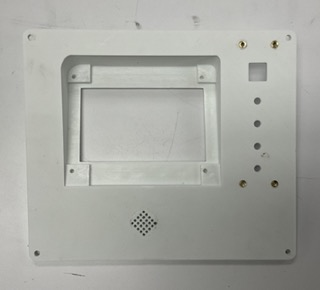
\includegraphics[width=\textwidth]{graphics/Empty Lid.jpeg}
            \caption{Heat Inserts In the Lid}
            \label{fig:Lid Heat Inserts}
        \end{subfigure}
        \begin{subfigure}{.45\textwidth}
            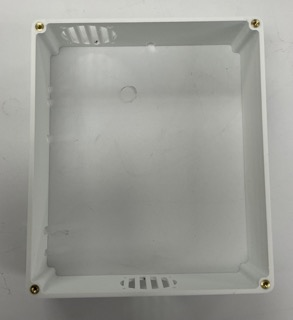
\includegraphics[width=\textwidth]{graphics/Enclosure Walls.jpeg}
            \caption{Heat Inserts In the Walls}
            \label{fig:Lid Heat Inserts 2}
        \end{subfigure}
    \end{figure}
\pagebreak
\subsection{Attaching Key Card Reader}
Due to the variance in screw hole placement on different brands of key card scanners, the holes must be manually marked and drilled for each assembly. First, place chosen scanner on a piece of paper and mark the screw hole placement by pushing a marker or pen through the paper and into the holes. Next, place the paper on the outside of the right enclosure wall (see photo) and mark the hole placement using the guide. Then drill out the holes with a bit corresponding with the size of the scanner's screws. 
Finally, screw the scanner into place on the outside of the enclosure walls with 3/8in 4/40 screws and with 2 washers on each screw, threading the screws from inside the wall through to the scanner.
\begin{figure}[H]
        \centering
        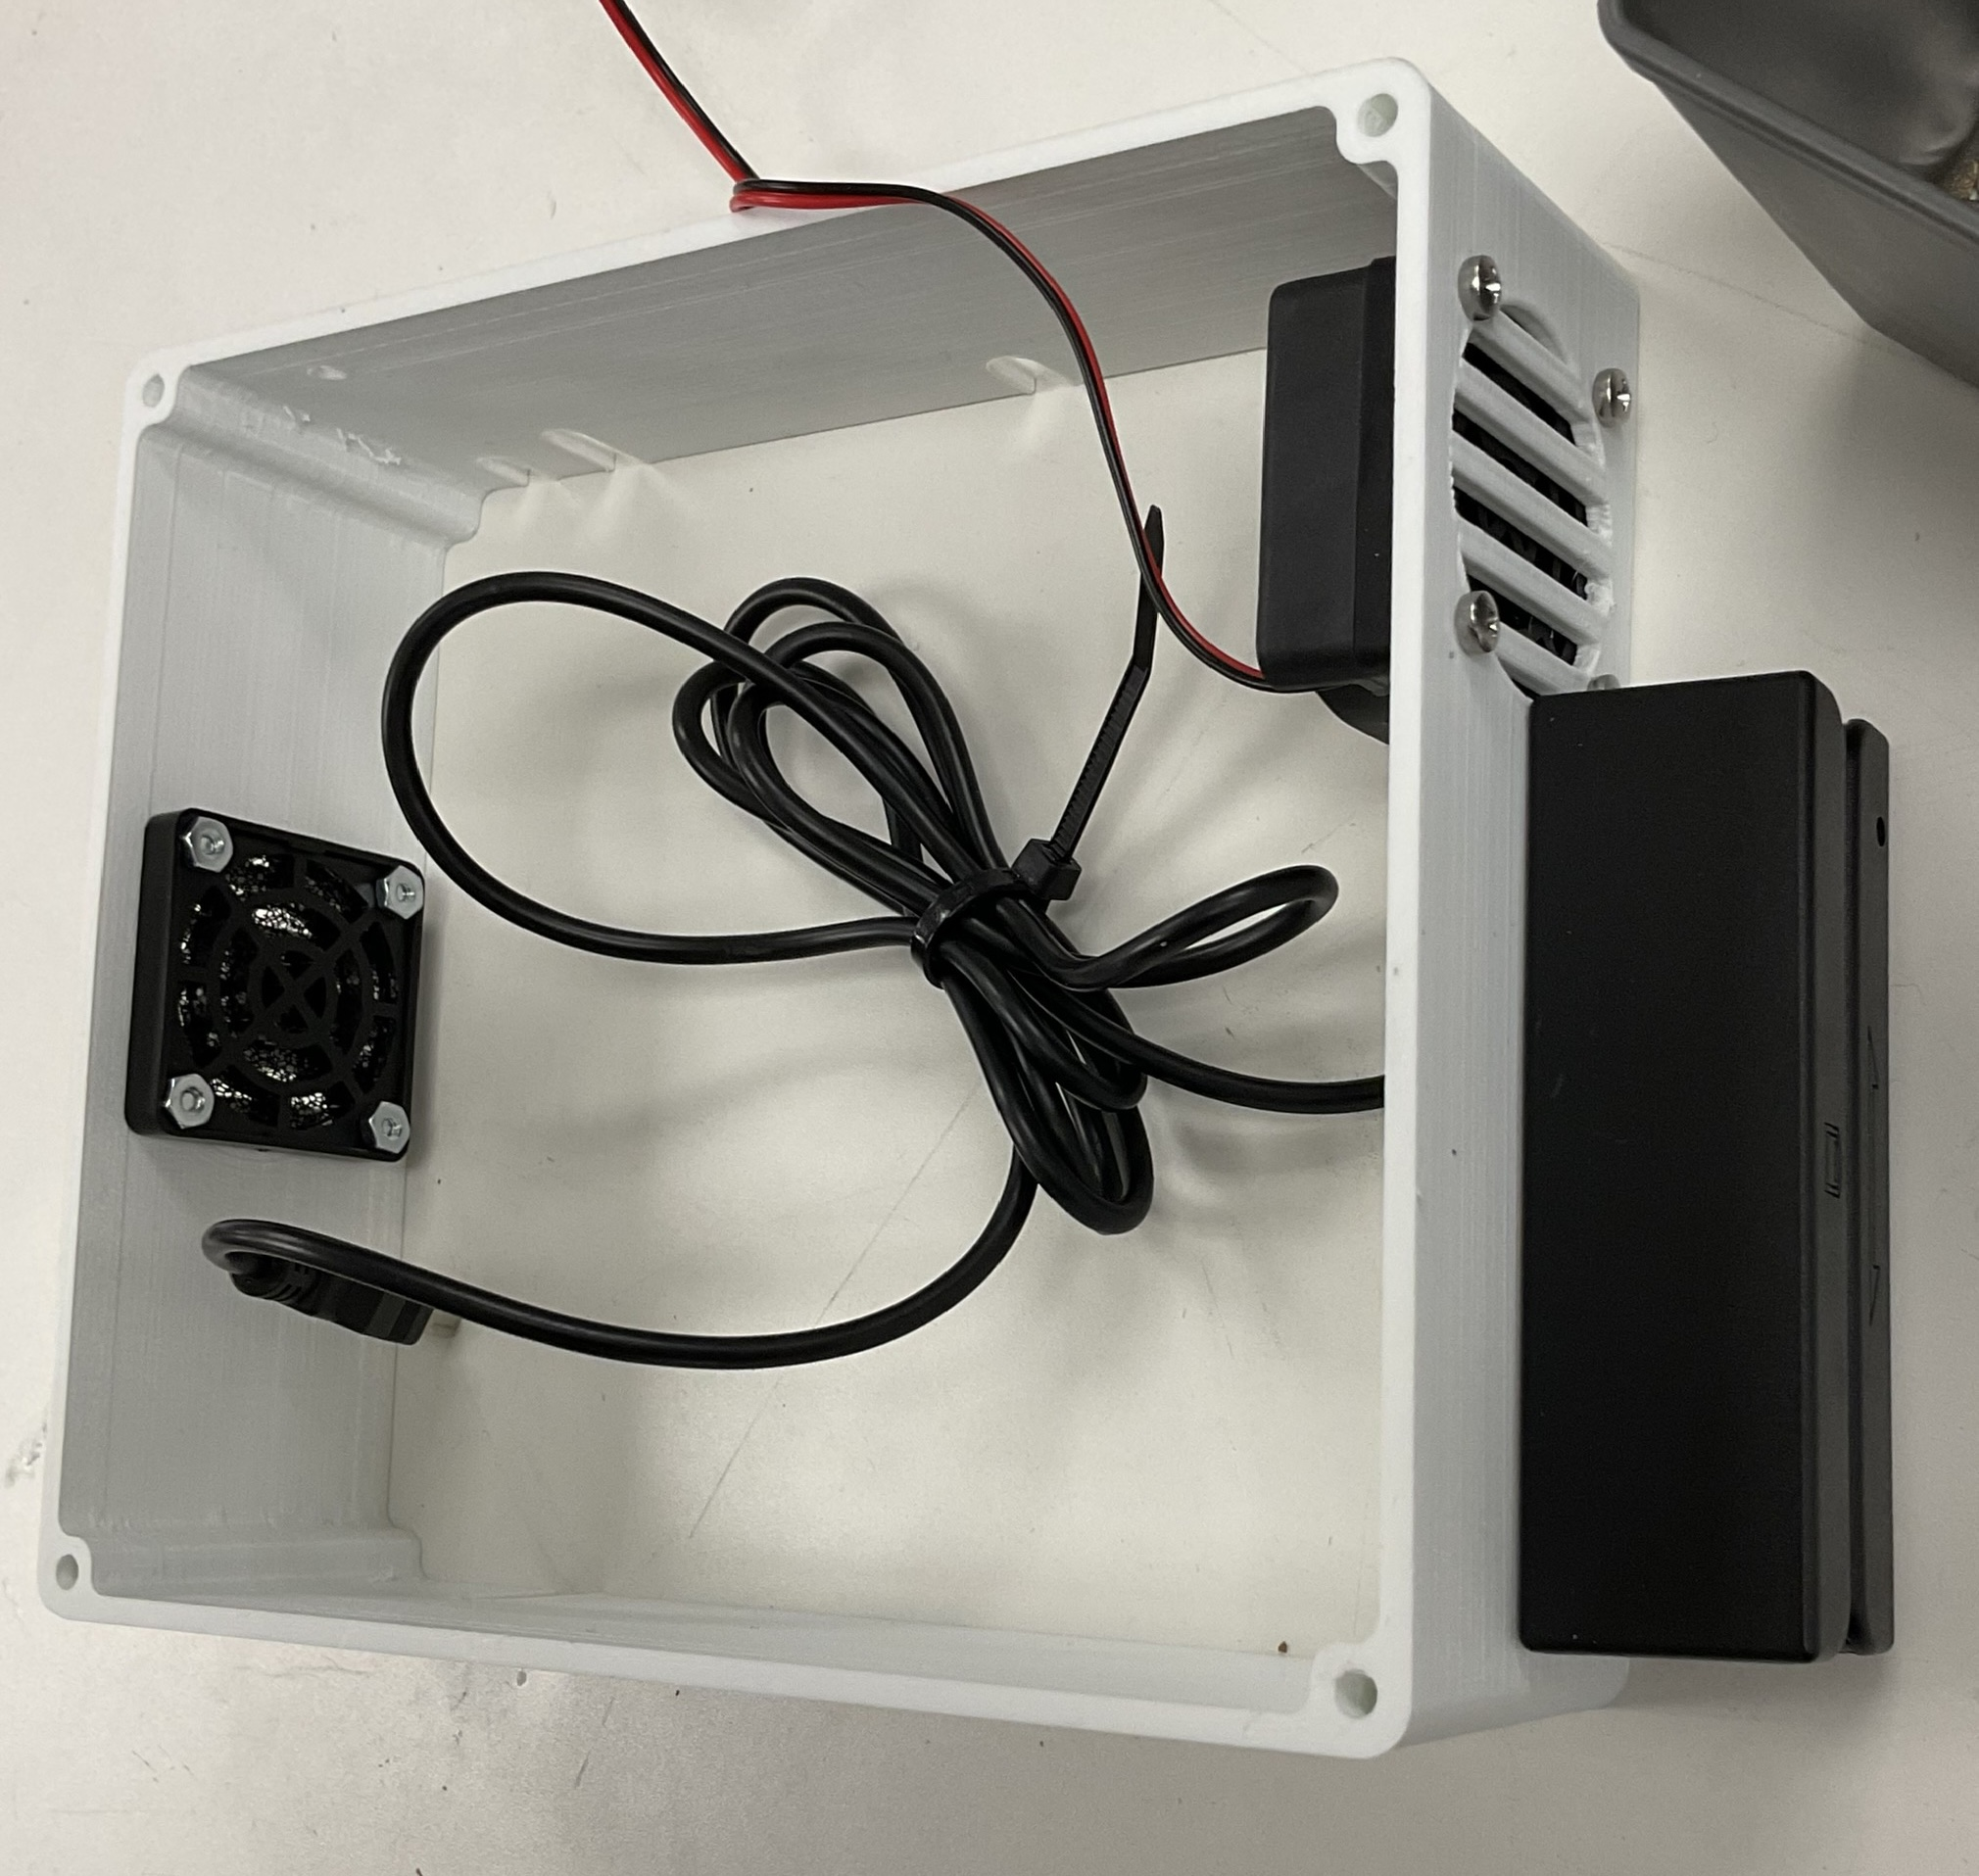
\includegraphics[width=.5\textwidth]{graphics/Scanner.jpg}
        \caption{Scanner Attached to Enclosure}
        \label{fig:Scanner}
    \end{figure}
\pagebreak
\subsection{Securing Internals}
The main PCB will be placed on top of the Raspberry Pi by connecting the headers, with metal standoffs in between, placed at each of the screw holes. The 12mm M2.5 screws go through the holes on the bottom of the case and into the threaded standoffs in between the boards. M2.5 are inserted through the top of the main PCB and into the standoffs to secure both boards. The vent filters and fans can be attached to either vent on the inside of the enclosure walls using 4/40 screws, inserting the screw from outside the walls, through the fan and/or filter, and using a nut to secure. Then the fan's cable can be connected to the main PCB. Finally, connect all cables to their correct ports, add strain relief with plastic zip ties, and wrap and secure the excess cable from the scanner.
    \begin{figure}[H]
        \centering
        \begin{subfigure}{.45\textwidth}
            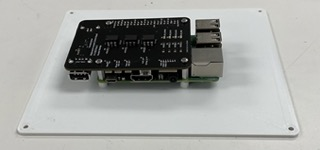
\includegraphics[width=\textwidth]{graphics/Bottom Internals.jpeg}
            \caption{Raspberry Pi and PCB Attached to Bottom Plate}
            \label{fig:Bottom Internals}
        \end{subfigure}
        \begin{subfigure}{.45\textwidth}
            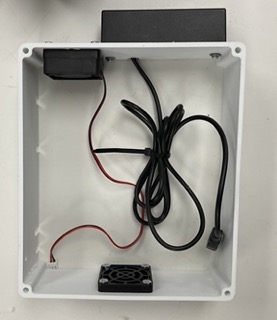
\includegraphics[width=\textwidth]{graphics/Fans.jpeg}
            \caption{Fans and Filters Attached to Walls}
            \label{fig:Bottom Internals 2}
        \end{subfigure}
    \end{figure}
\pagebreak
\subsection{Attaching Enclosure Walls}
After the cables have been connected to the correct ports and properly managed, the enclosure walls can be placed on top, ensuring the cables thread through the notches. Using the correct screws(3mm), the bottom enclosure plate can be secured to the walls by inserting the screws up through the bottom and into the walls.
\begin{figure}[H]
        \centering
        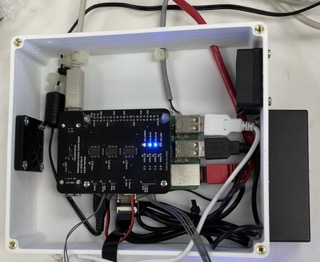
\includegraphics[width=.5\textwidth]{graphics/Internals Cables.jpeg}
        \caption{Cable Connections and Strain Relief}
        \label{fig:Cables}
    \end{figure}
\pagebreak
\subsection{Securing Lid and Connections}
The holes on the underside of the lid for the display must first be tapped using a 4-40 tap. Then the display can be screwed into place with the screws that come with them, ensuring the HDMI port is facing down. The secondary PCB can also be screwed into place on the underside of the lid with 4mm spacers in between the board and the lid to maintain the proper height. After both the HDMI cable and secondary board cable are connected to the main PCB and Raspberry Pi, the lid can be placed on top of the enclosure walls and secured in place with the 3mm security torx screws.
    \begin{figure}[H]
        \centering
        \begin{subfigure}{.45\textwidth}
            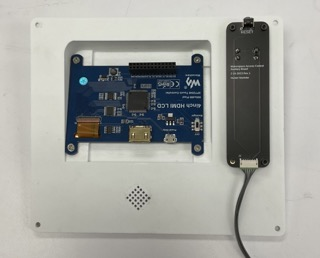
\includegraphics[width=\textwidth]{graphics/Lid Internals.jpeg}
            \caption{Display and Secondary PCB Attached to Lid}
            \label{fig:Lid Internals}
        \end{subfigure}
        \begin{subfigure}{.45\textwidth}
            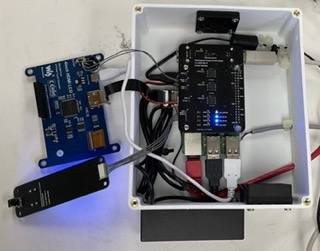
\includegraphics[width=\textwidth]{graphics/Internals Connections.jpeg}
            \caption{Cable Connections For All Internals}
            \label{fig:Final Cable Connections}
        \end{subfigure}
    \end{figure}
\subsection{Connecting to device}
Different devices will require different control methods. If it is a simple device that can just use USB then you just need to plug the USB line that plugs into the device into the controlling USB on the Main Board. If the device has a control line you will need the electrical schematic for that device and then find the door lines or another line that will pause the machine and then plug that line into our safety line control cable. If it is an AC-powered device then you will need to use a solid-state relay with a 3-5v control input voltage and then wire the power into that of whatever device you are trying to control as explained in \cref{sec: relay-controller}.